\documentclass{standalone}
\usepackage{tikz}
%\usetikzlibrary{...}
\begin{document}
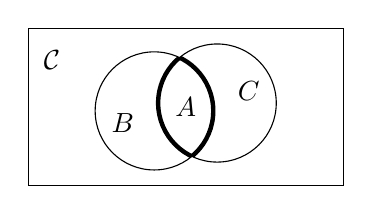
\begin{tikzpicture}
\draw (0,-2) rectangle (4,0);
\node (clab) at (0.3,-0.4) {$\mathcal{C}$};
\def\circleb{(1.6,-1.05) circle (0.75)}
\def\circlec{(2.4,-0.95) circle (0.75)}
\draw \circleb;
\draw \circlec;
\begin{scope}
   \clip \circleb;
   \draw[ultra thick] \circlec;
\end{scope}
\begin{scope}
   \clip \circlec;
   \draw[ultra thick] \circleb;
\end{scope}
\node at (2.0,-1.0) {$A$};
\node at (1.2,-1.2) {$B$};
\node at (2.8,-0.8) {$C$};
\end{tikzpicture}%
\end{document}
